\documentclass[tikz,border=10pt]{standalone}
\usepackage{pgfplots}
\pgfplotsset{compat=1.18}
\usetikzlibrary{arrows.meta, calc}

\begin{document}
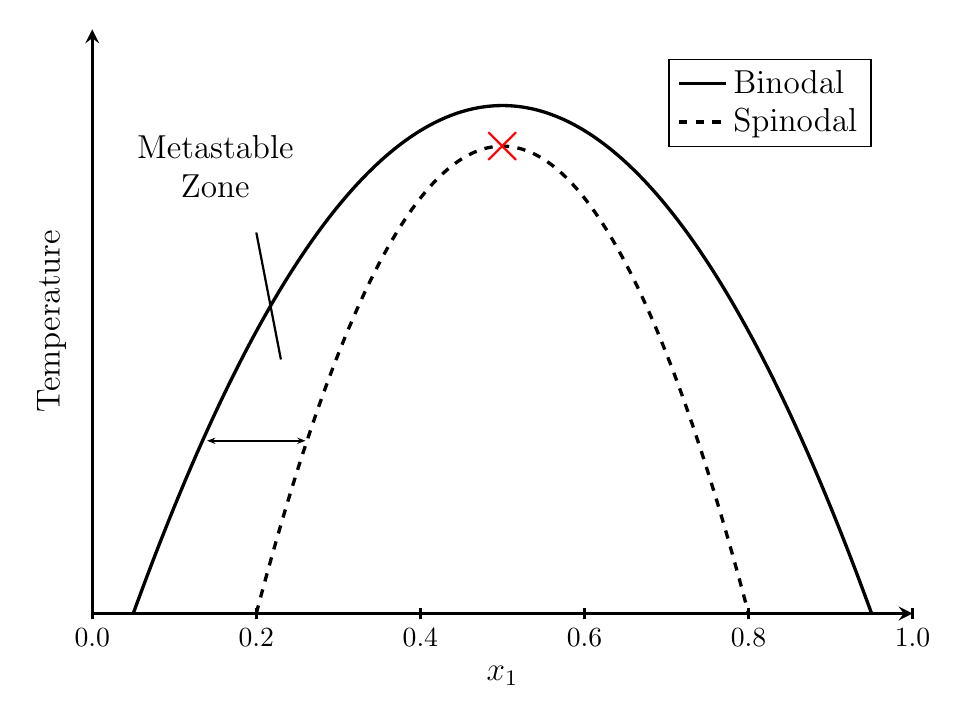
\begin{tikzpicture}
\begin{axis}[
    width=12cm,
    height=9cm,
    axis lines=left,
    xlabel={$x_1$},
    ylabel={Temperature},
    xlabel style={font=\large},
    ylabel style={font=\large, at={(axis description cs:-0.02,0.5)}},
    axis line style={very thick},
    xmin=0, xmax=1,
    ymin=0, ymax=1.15,
    xtick={0.0, 0.2, 0.4, 0.6, 0.8, 1.0},
    xticklabels={0.0, 0.2, 0.4, 0.6, 0.8, 1.0},
    ytick=\empty,
    clip=false,
    legend style={
        at={(0.95,0.95)},
        anchor=north east,
        draw=black,
        fill=white,
        font=\large,
        cells={anchor=west},
        legend cell align=left,
    },
    every tick/.style={very thick},
]

% --- Binodal curve (solid) ---
% Parabolic dome: zeros at x=0.05 and x=0.95, max ~1.0 at x=0.5
\addplot[
    black,
    very thick,
    solid,
    domain=0.05:0.95,
    samples=200,
] {4.938*(x - 0.05)*(0.95 - x)};
\addlegendentry{Binodal}

% --- Spinodal curve (dashed) ---
% Narrower dome: zeros at x=0.2 and x=0.8, max ~0.92 at x=0.5
\addplot[
    black,
    very thick,
    dashed,
    domain=0.2:0.8,
    samples=200,
] {10.222*(x - 0.2)*(0.8 - x)};
\addlegendentry{Spinodal}

% --- Red X at spinodal maximum (x=0.5, T~0.92) ---
\node[red, font=\Large\bfseries, scale=1.5] at (axis cs:0.5, 0.92) {$\times$};

% --- Metastable Zone annotation ---
% Text label in upper-left area
\node[font=\large, align=center] at (axis cs:0.15, 0.88) {Metastable\\Zone};

% Diagonal line from below label going down-right toward the crossing region
% Starts near (0.20, 0.75) and goes to about (0.23, 0.52)
\draw[thick] (axis cs:0.20, 0.75) -- (axis cs:0.23, 0.50);

% Horizontal double-arrow below, showing the metastable gap
% At T~0.34: binodal is at about x=0.14, spinodal at about x=0.26
\draw[thick, {Stealth[length=3pt]}-{Stealth[length=3pt]}]
    (axis cs:0.14, 0.34) -- (axis cs:0.26, 0.34);

\end{axis}
\end{tikzpicture}
\end{document}
